\chapter{the Dirac spinor}
\begin{itemize}
	\item 整个 Part \ref{part II} 中, 我们使用 $(+, -, -, -)$ 号差, 因为 $\mathrm{Cl}_{1, 3}(\mathbb{R}) \cancel{\simeq} \mathrm{Cl}_{3, 1}(\mathbb{R})$.
	
	\item 本笔记中的算符的定义与 A. Zee 的定义不同, 存在如下对应关系:
	
	\begin{center}
		\newcolumntype{K}{>{\centering\arraybackslash}X}
		\begin{tabularx}{\linewidth}{KK}
			\toprule 
			A. Zee's def. & my def. \\
			\midrule 
			$\omega_{\mu \nu}$ & $\omega_{\mu \nu}$ \\
			$- i J^{\mu \nu}$ & $J^{\mu \nu}$ \\
			$- i \sigma^{\mu \nu}$ & $\sigma^{\mu \nu}$ \\
			\bottomrule
		\end{tabularx}
	\end{center}
	
	\item $\Pi(\Lambda)$ 的写法可能不准确, (要考虑 universal cover, $\mathrm{Spin}(1, 3) \simeq \mathrm{Spin}(3, 1)$), 因为 Lorentz transform 对 spinor 的操作是 "path dependent", 因此本 chapter 中的 $\Lambda$ 都默认沿着以下的 path 做变换,
	\begin{equation}
		\Lambda(\lambda) = e^{\frac{\lambda}{2} \omega_{\mu \nu} J^{\mu \nu}}, \lambda \in [0, 1].
	\end{equation}
\end{itemize}

\section{gamma matrices}
\begin{itemize}
	\item Pauli 矩阵如下,
	\begin{equation}
		\sigma_1 = \begin{pmatrix}
			0 & 1 \\
			1 & 0
		\end{pmatrix}, \quad \sigma_2 = \begin{pmatrix}
			0 & - i \\
			i & 0
		\end{pmatrix}, \quad \sigma_3 = \begin{pmatrix}
			1 & 0 \\
			0 & - 1
		\end{pmatrix}.
	\end{equation}
	
	\item gamma 矩阵 (also called Dirac matrices) 如下 (其中 $i = 1, 2, 3$),
	\begin{equation}
		\gamma^0 = \begin{pmatrix}
			& I \\
			I &
		\end{pmatrix} = I \otimes \tau_1, \quad \gamma^i = \begin{pmatrix}
			& \sigma_i \\
			- \sigma_i &
		\end{pmatrix} = i \sigma_i \otimes \tau_2, \quad \gamma^5 = i \Omega = \begin{pmatrix}
			- I & \\
			& I
		\end{pmatrix} = - I \otimes \tau_3.
	\end{equation}
	其中 $\tau_{2, 3}$ 也是 Pauli 矩阵, $\Omega = \gamma^0 \gamma^1 \gamma^2 \gamma^3$, 有时候使用符号 $\sigma^\mu = (I, \vec{\sigma}), \bar{\sigma}^\mu = (I, - \vec{\sigma})$.
	\begin{itemize}
		\item 另外
		\begin{equation}
			\begin{dcases}
				\gamma^0 \gamma^i = - \sigma_i \otimes \tau_3 \\
				\gamma^i \gamma^j = - (\sigma_i \sigma_j) \otimes I = - i \epsilon_{i j k} \sigma_k \otimes I
			\end{dcases}, \quad \begin{dcases}
				\Omega \gamma^0 = - I \otimes \tau_2 \\
				\Omega \gamma^i = - \sigma_i \otimes \tau_2
			\end{dcases},
		\end{equation}
		其中, 用到了 $\sigma_i \sigma_j = i \epsilon_{i j k} \sigma_k$.
	\end{itemize}
	
	\noindent\rule[0.5ex]{\linewidth}{0.5pt} % horizontal line
	
	\item gamma 矩阵满足
	\begin{equation}
		\begin{dcases}
			(\gamma^\mu)^2 = \eta^{\mu \mu} \\
			\gamma^\mu \gamma^\nu = - \gamma^\nu \gamma^\mu & \mu \neq \nu
		\end{dcases} \Longrightarrow \{\gamma^\mu, \gamma^\nu\} = 2 \eta^{\mu \nu}.
	\end{equation}
	
	\item 且存在如下关系,
	\begin{align}
		& \Omega \gamma^0 = - \gamma^1 \gamma^2 \gamma^3, \quad \Omega \gamma^1 = - \gamma^0 \gamma^2 \gamma^3, \quad \Omega \gamma^2 = \gamma^0 \gamma^1 \gamma^3, \quad \Omega \gamma^3 = - \gamma^0 \gamma^1 \gamma^2, \notag \\
		\iff & - \tensor{\epsilon}{^{\mu \nu \rho}_\sigma} \Omega \gamma^\sigma = \gamma^\mu \gamma^\nu \gamma^\rho, \ \text{when} \ \mu \neq \nu \neq \rho.
	\end{align}
	并且有 (注意到 $\Omega^2 = - 1$),
	\begin{equation}
		\{\Omega, \gamma^\mu\} = 0, \quad \{\Omega, \Omega \gamma^\mu\} = 0, \quad [\Omega, \gamma^\mu \gamma^\nu] = 0.
	\end{equation}
	
	\noindent\hdashrule[0.5ex]{\linewidth}{0.5pt}{1mm} % horizontal dashed line
	
	\item 定义 $\sigma^{\mu \nu} = \frac{1}{2} [\gamma^\mu, \gamma^\nu]$ (注意, 我们的定义中没有虚数 $i$, 与 A. Zee 的定义不同), 因此
	\begin{equation}
		\gamma^\mu \gamma^\nu = \frac{1}{2} \{\gamma^\mu, \gamma^\nu\} + \frac{1}{2} [\gamma^\mu, \gamma^\nu] = \eta^{\mu \nu} + \sigma^{\mu \nu} \Longrightarrow \begin{dcases}
			\sigma^{0 i} = \begin{pmatrix}
				- \sigma_i & \\
				& \sigma_i
			\end{pmatrix} = - \sigma_i \otimes \tau_3 \\
			\sigma^{i j} = - i \epsilon^{i j k} \begin{pmatrix}
				\sigma_k & \\
				& \sigma_k
			\end{pmatrix} = - i \epsilon^{i j k} \sigma_k \otimes I
		\end{dcases},
	\end{equation}
	与笔记 \href{https://github.com/siyang03/my-note---Lie-Groups-and-Lie-Algebras}{Lie Groups and Lie Algebras} 中 $(\frac{1}{2}, 0) \oplus (0, \frac{1}{2})$ 表示对比, 可见 $\pi_{(\frac{1}{2}, 0) \oplus (0, \frac{1}{2})}(J^{\mu \nu}) = \frac{1}{2} \sigma^{\mu \nu}$.
\end{itemize}

\subsection{gamma matrices under Dirac basis}
\begin{itemize}
	\item 做如下相似变换 ($B = S^{- 1} A S$),
	\begin{equation} \label{6.1.8}
		S = \frac{\sqrt{2}}{2} \begin{pmatrix}
			I & - I \\
			I & I
		\end{pmatrix} \iff S^{- 1} = \frac{\sqrt{2}}{2} \begin{pmatrix}
			I & I \\
			- I & I
		\end{pmatrix},
	\end{equation}
	得到
	\begin{equation}
		\gamma^0 = \begin{pmatrix}
			I & \\
			& - I
		\end{pmatrix} = I \otimes \tau_3, \quad \gamma^i = \begin{pmatrix}
			& \sigma_i \\
			- \sigma_i &
		\end{pmatrix} = i \sigma_i \otimes \tau_2, \quad \gamma^5 = \begin{pmatrix}
			& I \\
			I &
		\end{pmatrix} = I \otimes \tau_1.
	\end{equation}
	
	\item 另外,
	\begin{equation}
		\begin{dcases}
			\gamma^0 \gamma^i = \sigma_i \otimes \tau_1 \\
			\gamma^i \gamma^j = - i \epsilon_{i j k} \sigma_k \otimes I
		\end{dcases}, \quad \begin{dcases}
			\Omega \gamma^0 = - I \otimes \tau_2 \\
			\Omega \gamma^i = i \sigma_i \otimes \tau_3
		\end{dcases},
	\end{equation}
	以及
	\begin{equation}
		\sigma^{0 i} = \begin{pmatrix}
			& \sigma_i \\
			\sigma_i &
		\end{pmatrix} = \sigma_i \otimes \tau_1, \quad \sigma^{i j} = - i \epsilon^{i j k} \begin{pmatrix}
			\sigma_k & \\
			& \sigma_k
		\end{pmatrix} = - i \epsilon^{i j k} \sigma_k \otimes I.
	\end{equation}
\end{itemize}

\section{Lorentz transformation and the \texorpdfstring{$(\frac{1}{2}, 0) \oplus (0, \frac{1}{2})$}{(1/2, 0)+(0, 1/2)} representation}
\begin{itemize}
	\item Lorentz 变换可以写成如下形式,
	\begin{equation}
		\Lambda = e^{\frac{1}{2} \omega_{\mu \nu} J^{\mu \nu}},
	\end{equation}
	其中 $\omega_{\mu \nu}$ 反对称, $J^{0 i}$ generate boosts and $J^{i j}$ generate rotations, (详见笔记 \href{https://github.com/siyang03/my-note---Lie-Groups-and-Lie-Algebras}{Lie Groups and Lie Algebras}).
	
	\begin{figure}[H]
		\centering
		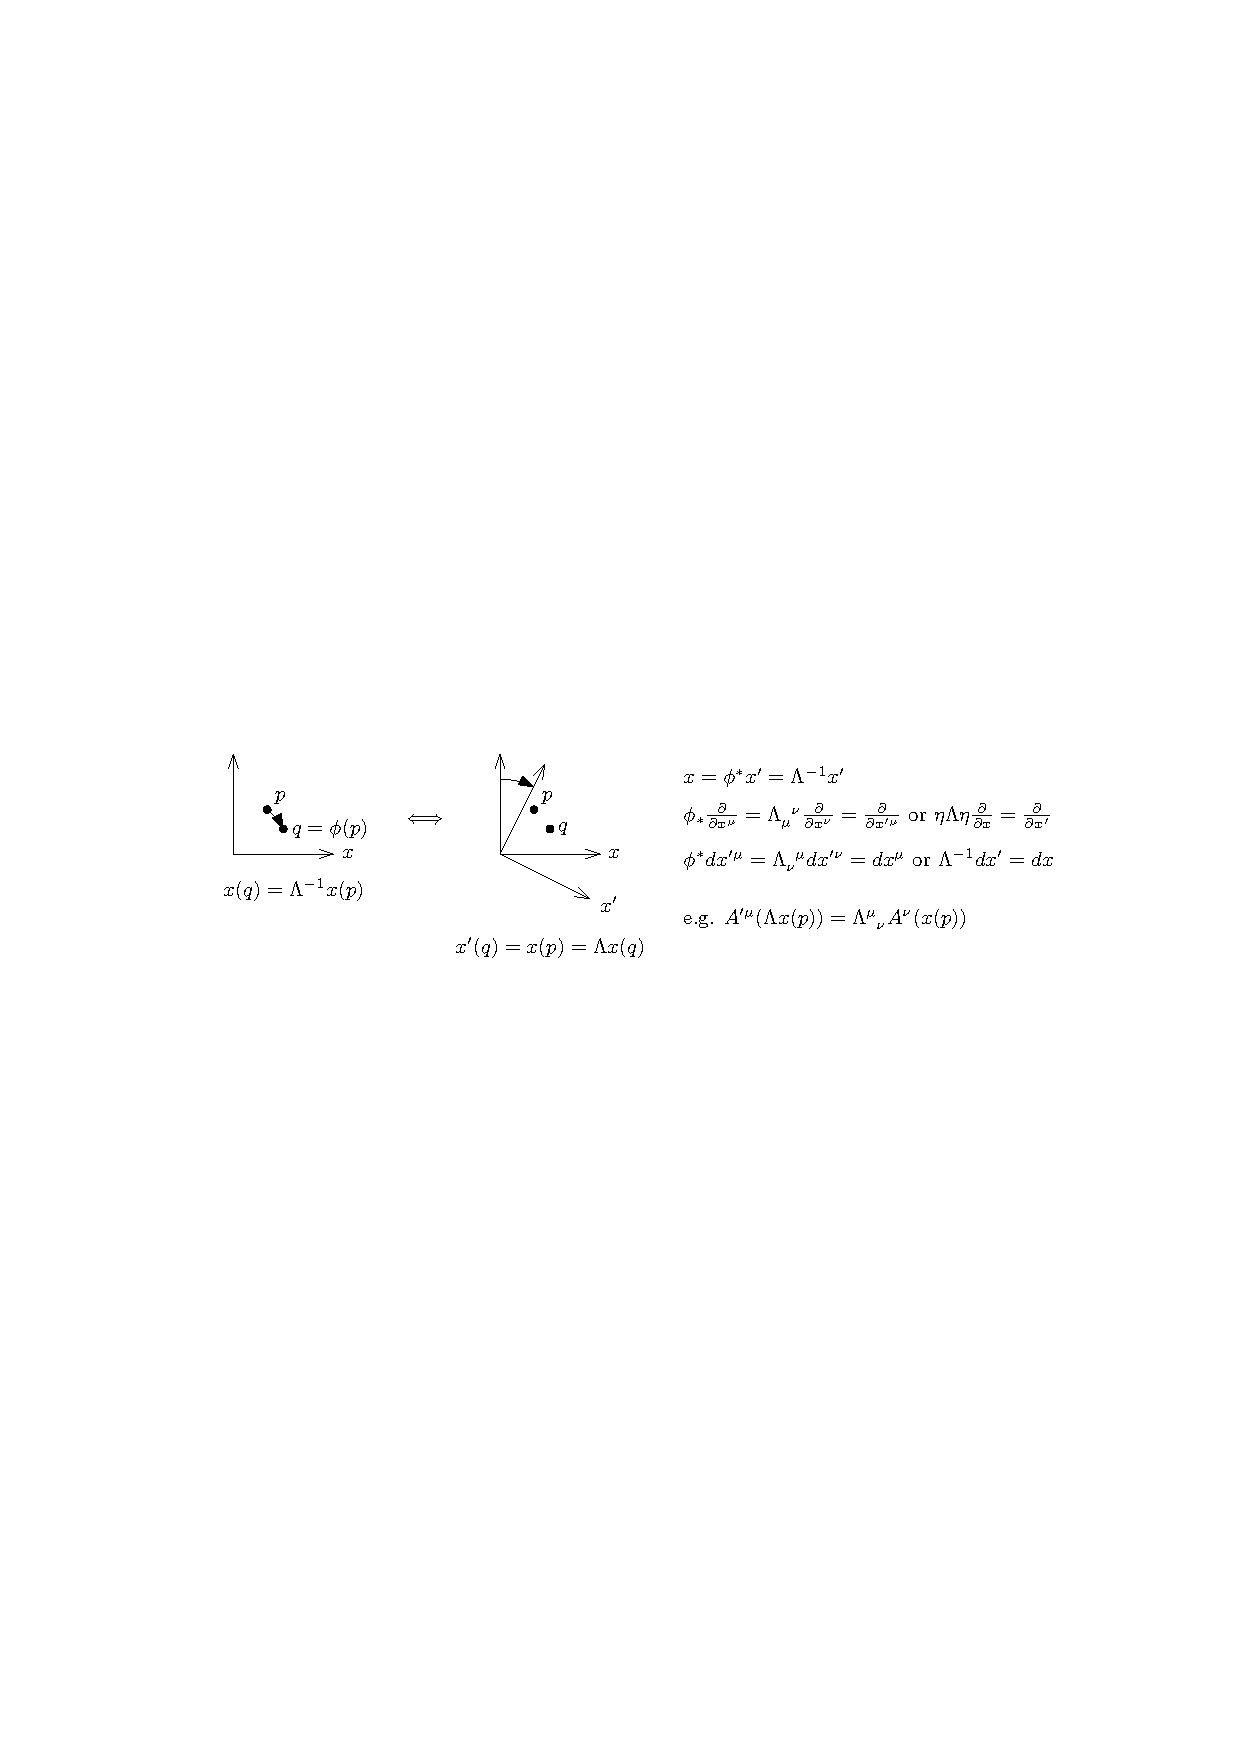
\includegraphics[scale=1]{figures/Lorentz transformation.pdf}
		\caption{Lorentz transformation}
	\end{figure}
	
	\noindent\rule[0.5ex]{\linewidth}{0.5pt} % horizontal line
	
	\item Weyl spinor 是 $(\frac{1}{2}, 0) \oplus (0, \frac{1}{2})$ rep. 的 vector space 中的元素,
	\begin{equation}
		\Psi = \begin{pmatrix}
			\psi_L \\
			\psi_R
		\end{pmatrix}, \quad \text{with} \quad \Psi_\text{Dirac} = S^{- 1} \Psi = \frac{\sqrt{2}}{2} \begin{pmatrix}
			\psi_L + \psi_R \\
			- \psi_L + \psi_R
		\end{pmatrix}.
	\end{equation}
	在 Weyl basis 下很容易看出,
	\begin{equation}
		\Psi_L = \underbrace{\frac{1}{2} (1 - \gamma^5)}_{= P_L} \Psi, \quad \Psi_R = \underbrace{\frac{1}{2} (1 + \gamma^5)}_{= P_R} \Psi.
	\end{equation}
	
	\noindent\rule[0.5ex]{\linewidth}{0.5pt} % horizontal line
	
	\item 对于 gamma 矩阵, 有
	\begin{equation}
		\Pi(\Lambda) \gamma^\rho \Pi^{- 1}(\Lambda) = e^{\frac{1}{4} \omega_{\mu \nu} \sigma^{\mu \nu}} \gamma^\rho e^{- \frac{1}{4} \omega_{\mu \nu} \sigma^{\mu \nu}} = \tensor{(\Lambda^{- 1})}{^\rho_\sigma} \gamma^\sigma.
	\end{equation}
	
	\begin{tcolorbox}[title=calculation:]
		利用 Campbell's identity,
		\begin{equation}
			e^{\frac{1}{4} \omega_{\mu \nu} \sigma^{\mu \nu}} \gamma^\rho e^{- \frac{1}{4} \omega_{\mu \nu} \sigma^{\mu \nu}} = e^{\frac{1}{4} \omega_{\mu \nu} \mathrm{ad}_{\sigma^{\mu \nu}}} \gamma^\rho,
		\end{equation}
		其中 (注意 $\tensor{(J^{\mu \nu})}{^\rho_\sigma} = 2 \eta^{[\mu| \rho} \tensor{\delta}{^{|\nu]}_\sigma}$, 其中度规号差与笔记 \href{https://github.com/siyang03/my-note---Lie-Groups-and-Lie-Algebras}{Lie Groups and Lie Algebras} 中的不同)
			\begin{align}
			& \begin{dcases}
				\rho \neq \mu, \nu & \begin{aligned}
					[\sigma^{\mu \nu}, \gamma^\rho] &= \frac{1}{2} (\gamma^\mu \gamma^\nu \gamma^\rho - \gamma^\nu \gamma^\mu \gamma^\rho - \gamma^\rho \gamma^\mu \gamma^\nu + \gamma^\rho \gamma^\nu \gamma^\mu) \\
					&= - \frac{1}{2} \underbrace{(\epsilon^{\mu \nu \rho \sigma} - \epsilon^{\nu \mu \rho \sigma} - \epsilon^{\rho \mu \nu \sigma} + \epsilon^{\rho \nu \mu \sigma})}_{= 0} \Omega \gamma_\sigma = 0
				\end{aligned} \\
				\rho = \mu \ \text{or} \ \nu \ \text{and} \ \mu \neq \nu & [\sigma^{\mu \nu}, \gamma^\rho] = 2 (\eta^{\mu \rho} \gamma^\mu - \eta^{\nu \rho} \gamma^\nu)
			\end{dcases} \notag \\
			\Longrightarrow & [\sigma^{\mu \nu}, \gamma^\rho] = 2 (\eta^{\nu \rho} \gamma^\mu - \eta^{\mu \rho} \gamma^\nu) = - 2 \tensor{(J^{\mu \nu})}{^\rho_\sigma} \gamma^\sigma,
		\end{align}
		代入, 得到
		\begin{equation}
			e^{\frac{1}{4} \omega_{\mu \nu} \mathrm{ad}_{\sigma^{\mu \nu}}} \gamma^\rho = \sum_{n = 0}^\infty \frac{1}{n!} \tensor{\Big( \Big( - \frac{1}{2} \omega_{\mu \nu} J^{\mu \nu} \Big)^n \Big)}{^\rho_\sigma} \gamma^\sigma = \tensor{(\Lambda^{- 1})}{^\rho_\sigma} \gamma^\sigma.
		\end{equation}
		
		\noindent\hdashrule[0.5ex]{\linewidth}{0.5pt}{1mm} % horizontal dashed line
		
		可以用 "无穷小" Lorentz 变换验证以上计算,
		\begin{align}
			\Pi(1 + \delta \tensor{\omega}{^\mu_\nu}) \gamma^\rho \Pi^{- 1}(1 + \delta \tensor{\omega}{^\mu_\nu}) &= \gamma^\rho + \frac{1}{4} \delta \omega_{\mu \nu} [\sigma^{\mu \nu}, \gamma^\rho] \notag \\
			&= (1 - \delta \tensor{\omega}{^\rho_\sigma}) \gamma^\sigma.
		\end{align}
	\end{tcolorbox}
\end{itemize}

\subsection{Dirac spinor}
\begin{itemize}
	\item 对于 Dirac spinor,
	\begin{equation}
		\Pi(\Lambda) \Psi(x) = \Psi'(\Lambda x),
	\end{equation}
	注意 $\partial'_\mu = \tensor{\Lambda}{_\mu^\nu} \partial_\nu$, 所以
	\begin{equation} \label{6.2.10}
		(i \gamma^\mu \partial_\mu - m) \Psi(x) = 0 \iff (i \gamma^\mu \partial'_\mu - m) \Psi'(\Lambda x) = 0.
	\end{equation}
	\begin{itemize}
		\item 关键部分在于
		\begin{equation}
			\gamma^\mu \Psi'(\Lambda x) = \gamma^\mu \Pi(\Lambda) \Psi(x) = \Pi(\Lambda) \tensor{\Lambda}{^\mu_\nu} \gamma^\nu \Psi(x).
		\end{equation}
	\end{itemize}
	
	\begin{tcolorbox}[title=calculation:]
		首先
		\begin{equation}
			\Lambda^T \eta \Lambda = \eta \Longrightarrow \tensor{(\Lambda^{- 1})}{^\mu_\nu} = \tensor{(\eta \Lambda^T \eta)}{^\mu_\nu} = \tensor{\Lambda}{_\nu^\mu},
		\end{equation}
		考虑
		\begin{equation}
			\Pi^{- 1}(\Lambda) \gamma^\mu \Pi(\Lambda) = \tensor{\Lambda}{^\mu_\nu} \gamma^\nu \Longrightarrow \gamma^\mu \Pi(\Lambda) = \tensor{\Lambda}{^\mu_\nu} \Pi(\Lambda) \gamma^\nu,
		\end{equation}
		代入,
		\begin{align}
			(i \gamma^\mu \partial'_\mu - m) \Psi'(\Lambda x) &= (i \gamma^\mu \tensor{\Lambda}{_\mu^\nu} \partial_\nu - m) \Pi(\Lambda) \Psi(x) \notag \\
			&= \Pi(\Lambda) (i \gamma^\rho \underbrace{\tensor{\Lambda}{^\mu_\rho} \tensor{\Lambda}{_\mu^\nu}}_{= \delta^\nu_\rho} \partial_\nu - m) \Psi(x) \notag \\
			&= \Pi(\Lambda) (i \gamma^\mu \partial_\mu - m) \Psi(x) = 0.
		\end{align}
	\end{tcolorbox}
\end{itemize}

\subsection{Dirac bilinears}
\begin{itemize}
	\item $\gamma^0$ 是 Hermitian 矩阵, 而 $\gamma^i$ 不是, 有
	\begin{equation} \label{6.2.15}
		\gamma^{i \dag} = - \gamma^i = \gamma^0 \gamma^i \gamma^0,
	\end{equation}
	可以统一写作 $\gamma^{\mu \dag} = \gamma^0 \gamma^\mu \gamma^0$, 并且有
	\begin{equation}
		\sigma^{\mu \nu \dag} = - \gamma^0 \sigma^{\mu \nu} \gamma^0, \quad \Pi^\dag(\Lambda) = \gamma^0 \Pi(\Lambda^{- 1}) \gamma^0.
	\end{equation}
	
	\begin{tcolorbox}[title=calculation:]
		对于 $\sigma^{\mu \nu}$,
		\begin{equation}
			\sigma^{\mu \nu \dag} = \frac{1}{2} (\gamma^{\nu \dag} \gamma^{\mu \dag} - \gamma^{\mu \dag} \gamma^{\nu \dag}) = \gamma^0 \sigma^{\mathcolor{red}{\nu \mu}} \gamma^0 = - \gamma^0 \sigma^{\mu \nu} \gamma^0,
		\end{equation}
		所以
		\begin{equation}
			((\omega_{\mu \nu} \sigma^{\mu \nu})^\dag)^n = \gamma^0 (- \omega_{\mu \nu} \sigma^{\mu \nu})^n \gamma^0 \Longrightarrow \Pi^\dag(\Lambda) = \gamma^0 \Pi(\Lambda^{- 1}) \gamma^0.
		\end{equation}
	\end{tcolorbox}
	
	\item 所以
	\begin{equation} \label{6.2.19}
		\begin{dcases}
			\bar{\Psi}'(\Lambda x) \Psi'(\Lambda x) = \bar{\Psi} \Psi & \text{scalar field} \\
			\bar{\Psi}' \gamma^\mu \Psi' = \tensor{\Lambda}{^\mu_\nu} \bar{\Psi} \gamma^\nu \Psi & \text{vector field}
		\end{dcases},
	\end{equation}
	其中 $\bar{\Psi} = \Psi^\dag \gamma^0$.
	
	\begin{tcolorbox}[title=calculation:]
		\begin{equation}
			\begin{dcases}
				\Psi'^\dag(\Lambda x) \gamma^0 \Psi'(\Lambda x) = \Psi^\dag(x) \gamma^0 \Pi(\Lambda^{- 1}) (\gamma^0)^2 \Pi(\Lambda) \Psi(x) = \Psi^\dag \gamma^0 \Psi \\
				\Psi'^\dag \gamma^0 \gamma^\mu \Psi' = \Psi^\dag(x) \gamma^0 \Pi(\Lambda^{- 1}) (\gamma^0)^2 \gamma^\mu \Pi(\Lambda) \Psi(x) = \tensor{\Lambda}{^\mu_\nu} \Psi^\dag \gamma^0 \gamma^\nu \Psi
			\end{dcases}.
		\end{equation}
		
		\noindent\rule[0.5ex]{\linewidth}{0.5pt} % horizontal line
		
		此外
		\begin{equation} \label{6.2.21}
			\begin{dcases}
				\bar{\Psi}' \sigma^{\mu \nu} \Psi' = \Psi^\dag \gamma^0 \Pi(\Lambda^{- 1}) (\gamma^0)^2 \sigma^{\mu \nu} \Pi(\Lambda) \Psi = \tensor{\Lambda}{^\mu_\rho} \tensor{\Lambda}{^\nu_\sigma} \bar{\Psi} \sigma^{\rho \sigma} \Psi & \text{order 2 tensor} \\
				\bar{\Psi}' \Omega \gamma^\mu \Psi' = \bar{\Psi} \Pi(\Lambda^{- 1}) \Omega \gamma^\mu \Pi(\Lambda) \Psi = \det(\Lambda) \tensor{\Lambda}{^\mu_\nu} \bar{\Psi} \Omega \gamma^\nu \Psi & \text{pseudovector} \\
				\bar{\Psi}' \Omega \Psi' = \bar{\Psi} \Pi(\Lambda^{- 1}) \Omega \Pi(\Lambda) \Psi = \det(\Lambda) \bar{\Psi} \Omega \Psi & \text{4-form (pseudoscalar)}
			\end{dcases},
		\end{equation}
		其中 (注意到下面的计算中, 第二个等号后, 含 $\eta$ 的项都等于零; 由此可以看出, 对 $\mu_i$ 求和的过程中, 任何两个 $\mu_i, \mu_j$ 相等的项求和之后都等于零)
		\begin{align}
			\Pi(\Lambda^{- 1}) \Omega \Pi(\Lambda) &= \prod_{i = 0}^3 \tensor{\Lambda}{^i_{\mu_i}} \gamma^{\mu_0} \gamma^{\mu_1} \gamma^{\mu_2} \gamma^{\mu_3} \notag \\
			&= \prod_{i = 0}^3 \tensor{\Lambda}{^i_{\mu_i}} (\eta^{\mu_0 \mu_1} + \sigma^{\mu_0 \mu_1}) (\eta^{\mu_2 \mu_3} + \sigma^{\mu_2 \mu_3}) \notag \\
			&= \prod_{i = 0}^3 \tensor{\Lambda}{^i_{\mu_i}} \gamma^{\mu_0} \gamma^{\mu_1} \gamma^{\mu_2} \gamma^{\mu_3} \quad \text{with} \quad \mu_0 \neq \mu_1 \neq \mu_2 \neq \mu_3 \notag \\
			&= \det(\Lambda) \Omega.
		\end{align}
	\end{tcolorbox}
\end{itemize}

\subsection{parity and time reversal}
\begin{itemize}
	\item 这里沿用笔记 \href{https://github.com/siyang03/my-note---Lie-Groups-and-Lie-Algebras}{Lie Groups and Lie Algebras} 中的记号, 选择 $\mathrm{O}(3, 1)$ 而非 $\mathrm{O}(1, 3)$, 因为他们没有区别.
	
	\item $\mathrm{O}(3, 1)$ 有 4 个联通分支,
	\begin{equation}
		I \in \mathrm{SO}_+(3, 1), \quad P T \in \mathrm{SO}_-(3, 1), \quad P \in \mathrm{O}'_+(3, 1), \quad T \in \mathrm{O}'_-(3, 1),
	\end{equation}
	其中
	\begin{equation}
		P = \mathrm{diag}(+ 1, - 1, - 1, - 1), \quad T = \mathrm{diag}(- 1, + 1, + 1, + 1),
	\end{equation}
	另外, $\eta P \eta = P, \eta T \eta = T$.
	
	\item 另外, Lorentz algebra 的 representation 不能自然的生成对 $P, T$ 的表示, 因为本质上它只能生成 spin group 的表示, 是 $\mathrm{SO}_+(3, 1)$ 的 universal cover, 与 Lorentz group 的其它三个连通分支没有直接联系.
	
	\item 因此, 对 $P, T$ 的表示要从物理的角度定义, (可能) 无法单纯靠数学的方法给出, 所以这部分放在下一章.
\end{itemize}
